\hypertarget{logfile_8h}{
\section{logfile.h File Reference}
\label{logfile_8h}\index{logfile.h@{logfile.h}}
}


This graph shows which files directly or indirectly include this file:\nopagebreak
\begin{figure}[H]
\begin{center}
\leavevmode
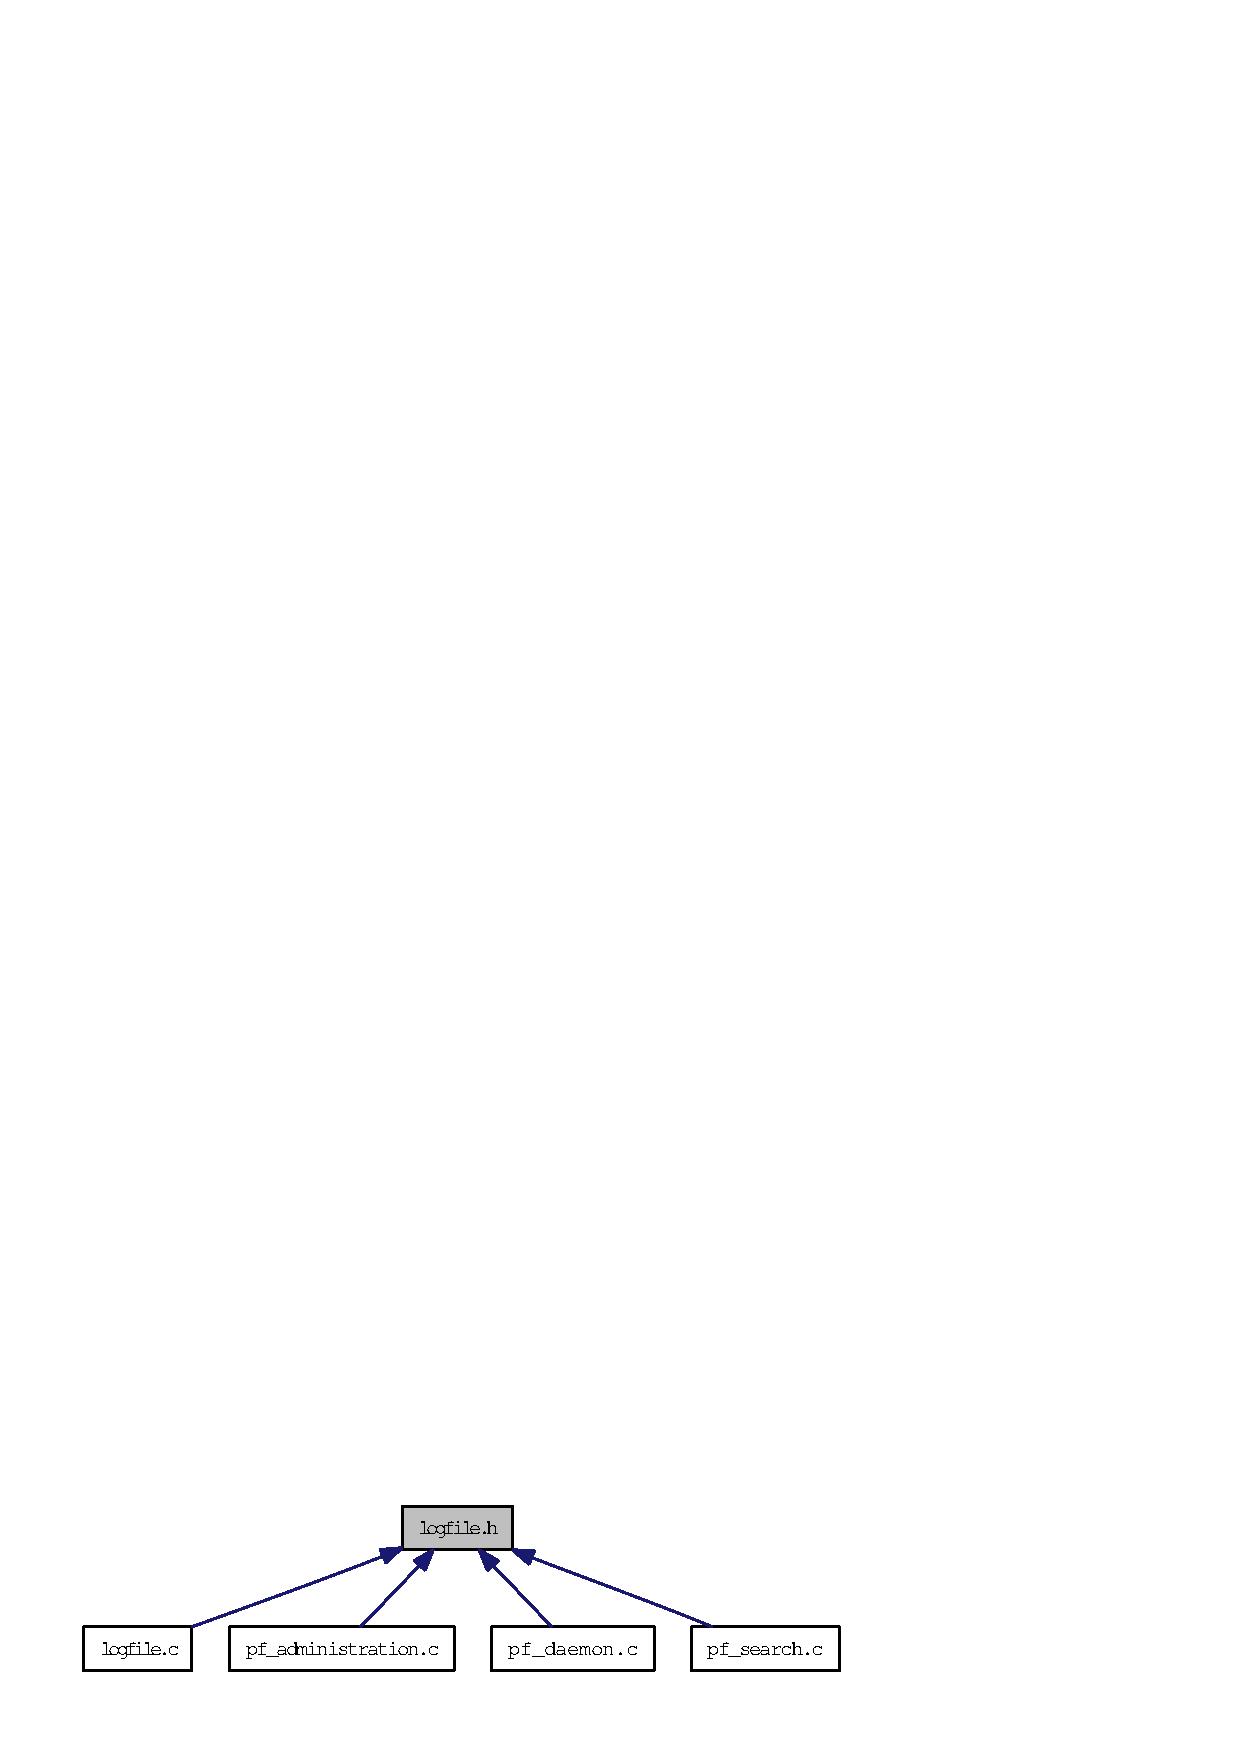
\includegraphics[width=135pt]{logfile_8h__dep__incl}
\end{center}
\end{figure}
\subsection*{Defines}
\begin{CompactItemize}
\item 
\#define \hyperlink{logfile_8h_6d3fef197146b932f5ad01fce683a66b}{LOGFILE}~\char`\"{}log/moksec.log\char`\"{}
\item 
\#define \hyperlink{logfile_8h_790d3f39336d5c73462ac5f113c79237}{MAX\_\-ENTRY\_\-LENGTH}~128
\item 
\#define \hyperlink{logfile_8h_c1ae4add974b9cfc6b5aaf8a578f01ab}{UNKNOWN}~0
\item 
\#define \hyperlink{logfile_8h_cd48c0293626a8577ef1c28ad58ca0d6}{ERR\_\-FLAG}~1
\item 
\#define \hyperlink{logfile_8h_d683e726fb2cb177c24b8cb84e80ea7d}{WARN\_\-FLAG}~2
\item 
\#define \hyperlink{logfile_8h_655cb5e43527221af659a76352b141ae}{INFO\_\-FLAG}~3
\item 
\#define \hyperlink{logfile_8h_33f75163eff20214d9f9a009d0d98096}{UNKNOWN\_\-LOG}(m)~write\_\-logentry(m, COMPONENT\_\-NAME, UNKNOWN\_\-FLAG)
\item 
\#define \hyperlink{logfile_8h_41569958738d77fee8d8ee52645a581b}{ERR\_\-LOG}(m)~write\_\-logentry(m, COMPONENT\_\-NAME, ERR\_\-FLAG)
\item 
\#define \hyperlink{logfile_8h_cf6e906d16742b29defc431585917af0}{WARN\_\-LOG}(m)~write\_\-logentry(m, COMPONENT\_\-NAME, WARN\_\-FLAG)
\item 
\#define \hyperlink{logfile_8h_5f7fc5ef70b11517748aa589e4128f61}{INFO\_\-LOG}(m)~write\_\-logentry(m, COMPONENT\_\-NAME, INFO\_\-FLAG)
\end{CompactItemize}
\subsection*{Functions}
\begin{CompactItemize}
\item 
int \hyperlink{logfile_8h_f71f5daf2025b4e30a18ccedf7c34863}{write\_\-logentry} (char $\ast$msg, char $\ast$component, int flag)
\end{CompactItemize}


\subsection{Define Documentation}
\hypertarget{logfile_8h_cd48c0293626a8577ef1c28ad58ca0d6}{
\index{logfile.h@{logfile.h}!ERR\_\-FLAG@{ERR\_\-FLAG}}
\index{ERR\_\-FLAG@{ERR\_\-FLAG}!logfile.h@{logfile.h}}
\subsubsection{\setlength{\rightskip}{0pt plus 5cm}\#define ERR\_\-FLAG~1}}
\label{logfile_8h_cd48c0293626a8577ef1c28ad58ca0d6}




Definition at line 25 of file logfile.h.

Referenced by write\_\-logentry().\hypertarget{logfile_8h_41569958738d77fee8d8ee52645a581b}{
\index{logfile.h@{logfile.h}!ERR\_\-LOG@{ERR\_\-LOG}}
\index{ERR\_\-LOG@{ERR\_\-LOG}!logfile.h@{logfile.h}}
\subsubsection{\setlength{\rightskip}{0pt plus 5cm}\#define ERR\_\-LOG(m)~write\_\-logentry(m, COMPONENT\_\-NAME, ERR\_\-FLAG)}}
\label{logfile_8h_41569958738d77fee8d8ee52645a581b}




Definition at line 30 of file logfile.h.

Referenced by add\_\-entry(), check\_\-entry(), get\_\-entry\_\-by\_\-name(), get\_\-entry\_\-by\_\-number(), get\_\-entry\_\-by\_\-reason(), and rm\_\-entry().\hypertarget{logfile_8h_655cb5e43527221af659a76352b141ae}{
\index{logfile.h@{logfile.h}!INFO\_\-FLAG@{INFO\_\-FLAG}}
\index{INFO\_\-FLAG@{INFO\_\-FLAG}!logfile.h@{logfile.h}}
\subsubsection{\setlength{\rightskip}{0pt plus 5cm}\#define INFO\_\-FLAG~3}}
\label{logfile_8h_655cb5e43527221af659a76352b141ae}




Definition at line 27 of file logfile.h.

Referenced by write\_\-logentry().\hypertarget{logfile_8h_5f7fc5ef70b11517748aa589e4128f61}{
\index{logfile.h@{logfile.h}!INFO\_\-LOG@{INFO\_\-LOG}}
\index{INFO\_\-LOG@{INFO\_\-LOG}!logfile.h@{logfile.h}}
\subsubsection{\setlength{\rightskip}{0pt plus 5cm}\#define INFO\_\-LOG(m)~write\_\-logentry(m, COMPONENT\_\-NAME, INFO\_\-FLAG)}}
\label{logfile_8h_5f7fc5ef70b11517748aa589e4128f61}




Definition at line 32 of file logfile.h.

Referenced by check\_\-entry().\hypertarget{logfile_8h_6d3fef197146b932f5ad01fce683a66b}{
\index{logfile.h@{logfile.h}!LOGFILE@{LOGFILE}}
\index{LOGFILE@{LOGFILE}!logfile.h@{logfile.h}}
\subsubsection{\setlength{\rightskip}{0pt plus 5cm}\#define LOGFILE~\char`\"{}log/moksec.log\char`\"{}}}
\label{logfile_8h_6d3fef197146b932f5ad01fce683a66b}




Definition at line 21 of file logfile.h.

Referenced by write\_\-logentry().\hypertarget{logfile_8h_790d3f39336d5c73462ac5f113c79237}{
\index{logfile.h@{logfile.h}!MAX\_\-ENTRY\_\-LENGTH@{MAX\_\-ENTRY\_\-LENGTH}}
\index{MAX\_\-ENTRY\_\-LENGTH@{MAX\_\-ENTRY\_\-LENGTH}!logfile.h@{logfile.h}}
\subsubsection{\setlength{\rightskip}{0pt plus 5cm}\#define MAX\_\-ENTRY\_\-LENGTH~128}}
\label{logfile_8h_790d3f39336d5c73462ac5f113c79237}




Definition at line 22 of file logfile.h.

Referenced by write\_\-logentry().\hypertarget{logfile_8h_c1ae4add974b9cfc6b5aaf8a578f01ab}{
\index{logfile.h@{logfile.h}!UNKNOWN@{UNKNOWN}}
\index{UNKNOWN@{UNKNOWN}!logfile.h@{logfile.h}}
\subsubsection{\setlength{\rightskip}{0pt plus 5cm}\#define UNKNOWN~0}}
\label{logfile_8h_c1ae4add974b9cfc6b5aaf8a578f01ab}




Definition at line 24 of file logfile.h.

Referenced by write\_\-logentry().\hypertarget{logfile_8h_33f75163eff20214d9f9a009d0d98096}{
\index{logfile.h@{logfile.h}!UNKNOWN\_\-LOG@{UNKNOWN\_\-LOG}}
\index{UNKNOWN\_\-LOG@{UNKNOWN\_\-LOG}!logfile.h@{logfile.h}}
\subsubsection{\setlength{\rightskip}{0pt plus 5cm}\#define UNKNOWN\_\-LOG(m)~write\_\-logentry(m, COMPONENT\_\-NAME, UNKNOWN\_\-FLAG)}}
\label{logfile_8h_33f75163eff20214d9f9a009d0d98096}




Definition at line 29 of file logfile.h.\hypertarget{logfile_8h_d683e726fb2cb177c24b8cb84e80ea7d}{
\index{logfile.h@{logfile.h}!WARN\_\-FLAG@{WARN\_\-FLAG}}
\index{WARN\_\-FLAG@{WARN\_\-FLAG}!logfile.h@{logfile.h}}
\subsubsection{\setlength{\rightskip}{0pt plus 5cm}\#define WARN\_\-FLAG~2}}
\label{logfile_8h_d683e726fb2cb177c24b8cb84e80ea7d}




Definition at line 26 of file logfile.h.

Referenced by write\_\-logentry().\hypertarget{logfile_8h_cf6e906d16742b29defc431585917af0}{
\index{logfile.h@{logfile.h}!WARN\_\-LOG@{WARN\_\-LOG}}
\index{WARN\_\-LOG@{WARN\_\-LOG}!logfile.h@{logfile.h}}
\subsubsection{\setlength{\rightskip}{0pt plus 5cm}\#define WARN\_\-LOG(m)~write\_\-logentry(m, COMPONENT\_\-NAME, WARN\_\-FLAG)}}
\label{logfile_8h_cf6e906d16742b29defc431585917af0}




Definition at line 31 of file logfile.h.

\subsection{Function Documentation}
\hypertarget{logfile_8h_f71f5daf2025b4e30a18ccedf7c34863}{
\index{logfile.h@{logfile.h}!write\_\-logentry@{write\_\-logentry}}
\index{write\_\-logentry@{write\_\-logentry}!logfile.h@{logfile.h}}
\subsubsection{\setlength{\rightskip}{0pt plus 5cm}int write\_\-logentry (char $\ast$ {\em msg}, char $\ast$ {\em component}, int {\em flag})}}
\label{logfile_8h_f71f5daf2025b4e30a18ccedf7c34863}


Writes a logfile enty.

\begin{Desc}
\item[Parameters:]
\begin{description}
\item[{\em msg}]The message which should be written in the logfile. \item[{\em component}]The program which calls the write\_\-logentry function, for example \char`\"{}phonefirewall\char`\"{} \item[{\em flag}]What message should be written. Use the defined flags.\end{description}
\end{Desc}
\begin{Desc}
\item[Returns:]-1 if something fails, otherwise 0 \end{Desc}


Definition at line 56 of file logfile.c.

References asctime(), ERR\_\-FLAG, INFO\_\-FLAG, LOGFILE, MAX\_\-ENTRY\_\-LENGTH, UNKNOWN, and WARN\_\-FLAG.

Here is the call graph for this function:\nopagebreak
\begin{figure}[H]
\begin{center}
\leavevmode
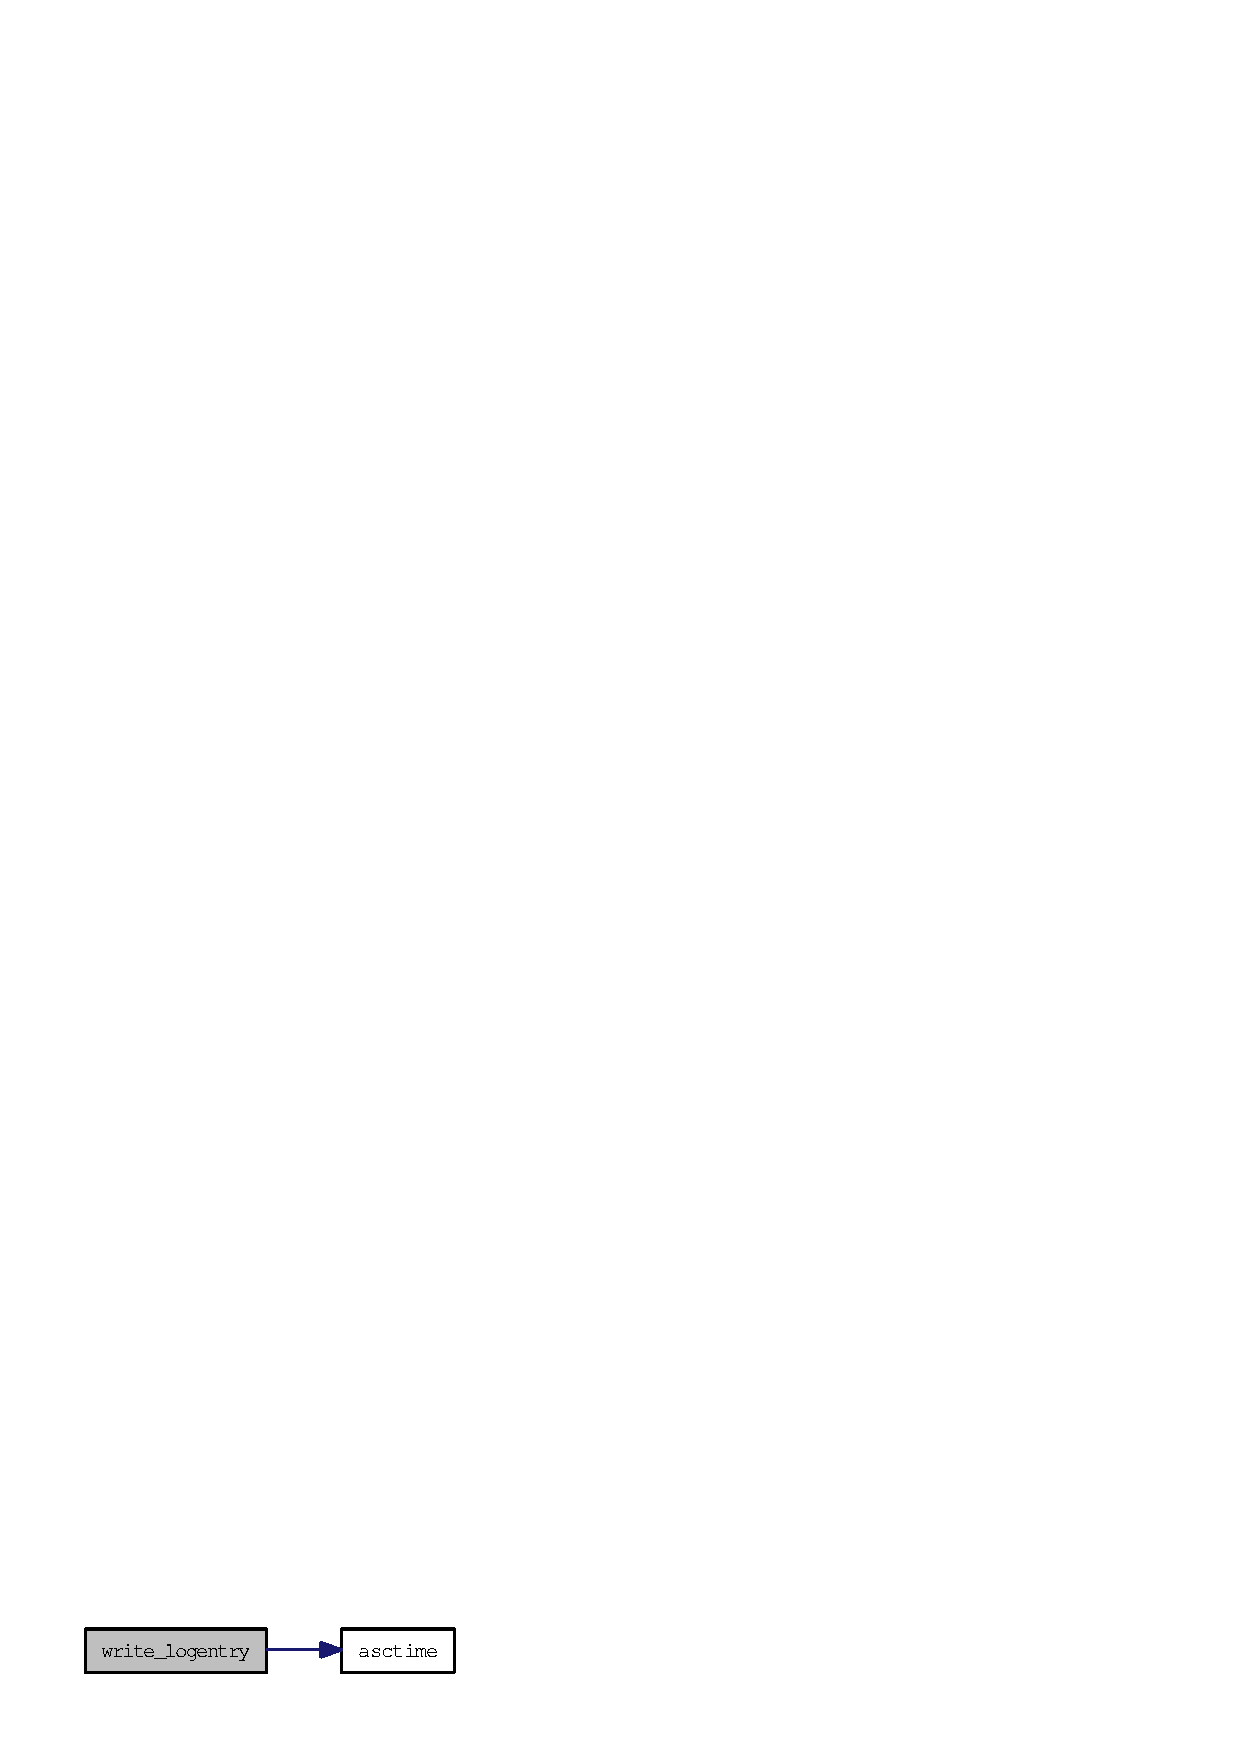
\includegraphics[width=111pt]{logfile_8h_f71f5daf2025b4e30a18ccedf7c34863_cgraph}
\end{center}
\end{figure}
